% Title: gl2ps_renderer figure
% Creator: GL2PS 1.4.2, (C) 1999-2020 C. Geuzaine
% For: Octave
% CreationDate: Tue Oct 26 15:58:46 2021
\setlength{\unitlength}{1pt}
\begin{picture}(0,0)
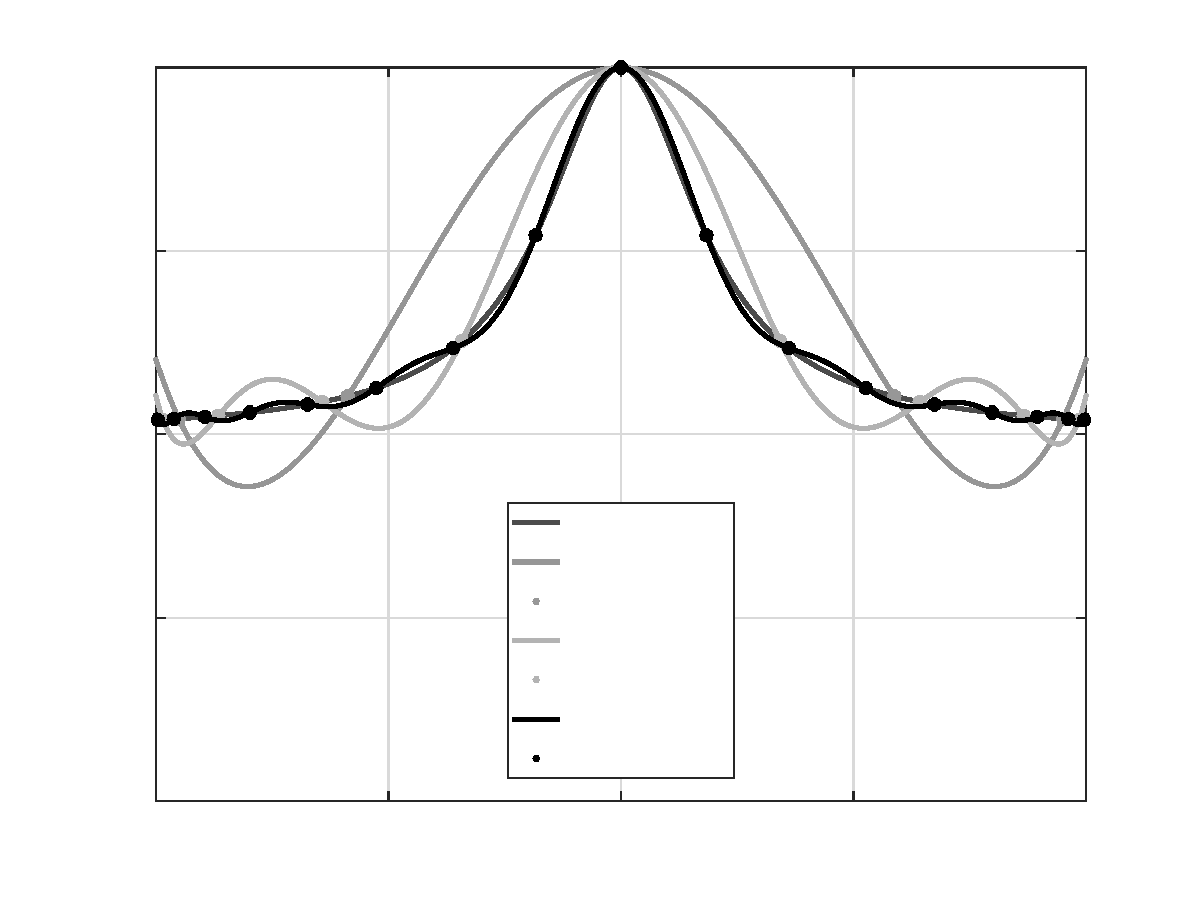
\includegraphics[scale=1]{OUT/RungePhenomFixGray-inc}
\end{picture}%
\begin{picture}(576,432)(0,0)
\fontsize{10}{0}\selectfont\put(74.8799,40.0181){\makebox(0,0)[t]{\textcolor[rgb]{0.15,0.15,0.15}{{-1}}}}
\fontsize{10}{0}\selectfont\put(186.48,40.0181){\makebox(0,0)[t]{\textcolor[rgb]{0.15,0.15,0.15}{{-0.5}}}}
\fontsize{10}{0}\selectfont\put(298.08,40.0181){\makebox(0,0)[t]{\textcolor[rgb]{0.15,0.15,0.15}{{0}}}}
\fontsize{10}{0}\selectfont\put(409.68,40.0181){\makebox(0,0)[t]{\textcolor[rgb]{0.15,0.15,0.15}{{0.5}}}}
\fontsize{10}{0}\selectfont\put(521.28,40.0181){\makebox(0,0)[t]{\textcolor[rgb]{0.15,0.15,0.15}{{1}}}}
\fontsize{10}{0}\selectfont\put(69.8755,47.52){\makebox(0,0)[r]{\textcolor[rgb]{0.15,0.15,0.15}{{-1}}}}
\fontsize{10}{0}\selectfont\put(69.8755,135.54){\makebox(0,0)[r]{\textcolor[rgb]{0.15,0.15,0.15}{{-0.5}}}}
\fontsize{10}{0}\selectfont\put(69.8755,223.56){\makebox(0,0)[r]{\textcolor[rgb]{0.15,0.15,0.15}{{0}}}}
\fontsize{10}{0}\selectfont\put(69.8755,311.58){\makebox(0,0)[r]{\textcolor[rgb]{0.15,0.15,0.15}{{0.5}}}}
\fontsize{10}{0}\selectfont\put(69.8755,399.6){\makebox(0,0)[r]{\textcolor[rgb]{0.15,0.15,0.15}{{1}}}}
\fontsize{11}{0}\selectfont\put(298.08,27.0181){\makebox(0,0)[t]{\textcolor[rgb]{0.15,0.15,0.15}{{$x$}}}}
\fontsize{9}{0}\selectfont\put(270.881,181.067){\makebox(0,0)[l]{\textcolor[rgb]{0,0,0}{{$f(x)$}}}}
\fontsize{9}{0}\selectfont\put(270.881,162.21){\makebox(0,0)[l]{\textcolor[rgb]{0,0,0}{{$p_4(x)$}}}}
\fontsize{9}{0}\selectfont\put(270.881,143.352){\makebox(0,0)[l]{\textcolor[rgb]{0,0,0}{{interpolation points}}}}
\fontsize{9}{0}\selectfont\put(270.881,124.494){\makebox(0,0)[l]{\textcolor[rgb]{0,0,0}{{$p_8(x)$}}}}
\fontsize{9}{0}\selectfont\put(270.881,105.637){\makebox(0,0)[l]{\textcolor[rgb]{0,0,0}{{interpolation points}}}}
\fontsize{9}{0}\selectfont\put(270.881,86.7788){\makebox(0,0)[l]{\textcolor[rgb]{0,0,0}{{$p_{16}(x)$}}}}
\fontsize{9}{0}\selectfont\put(270.881,67.9214){\makebox(0,0)[l]{\textcolor[rgb]{0,0,0}{{interpolation points}}}}
\end{picture}
